\subsection{M.PD.29 - Tolleranza agli errori}

\begin{figure}[H]
  \centering
  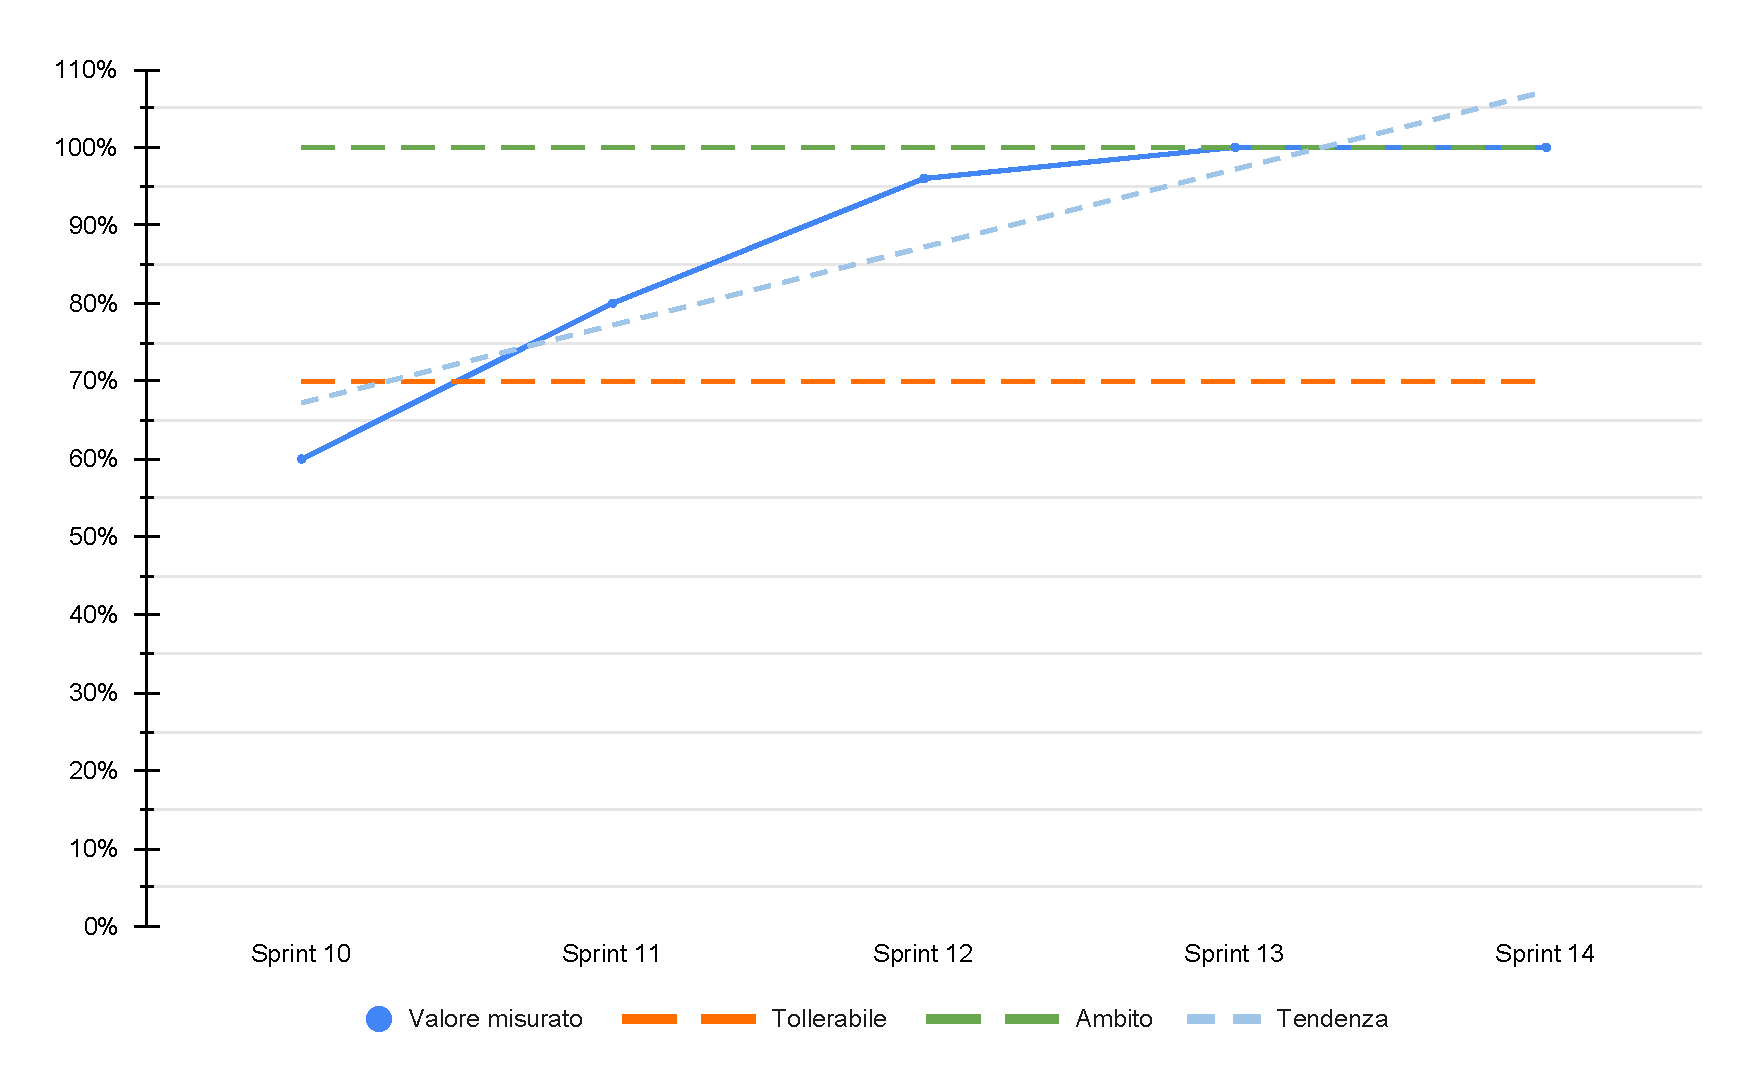
\includegraphics[width=\textwidth]{assets/tolleranza_errori.pdf}
  \caption{M.PD.19 - Tolleranza agli errori}
\end{figure}

\par La tolleranza agli errori è stata mantenuta su livelli alti sin dal primo sprint della \glossario{PB}, grazie all'implementazione del costrutto try-catch per gestire le eccezioni nel codice \glossario{front-end}. Durante lo \glossario{sprint} 11, il team ha introdotto una gestione centralizzata degli errori e rafforzato i controlli sui metodi che eseguono chiamate \glossario{API}. Questo ha consentito di migliorare la tolleranza, rientrando nel range di tollerabilità previsto. Successivamente, sono state sviluppate le funzionalità mancanti per la gestione degli errori, in particolare quelle relative alle operazioni \glossario{CRUD} sui \glossario{dizionari dati}. I test hanno inoltre evidenziato sezioni di codice che necessitavano dell'uso del costrutto try-catch. Dopo aver mitigato gli errori meno evidenti rilevati dai test, il team ha raggiunto una tolleranza del 100\%.